\documentclass{article}
\usepackage{tikz}
\usetikzlibrary{positioning,shapes.geometric}

% Define node styles
\tikzset{
  server/.style={draw, rounded corners=3pt, text width=15mm, minimum height=7mm},
  cache/.style={draw, circle, minimum size=12mm},
  request/.style={->, very thick, black!40},
  delay/.style={->, very thick, dashed, black!60}
}

\begin{document}

\begin{center}
    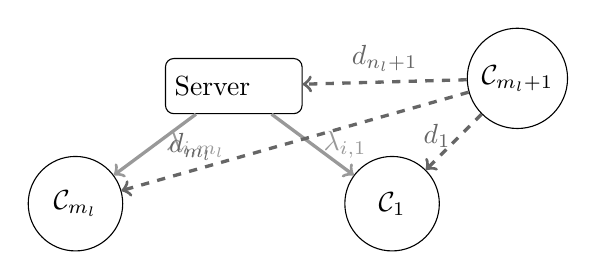
\begin{tikzpicture}[node distance=1cm]
        % Define nodes
        \node[server] (server) {Server};
        \node[cache, below right=of server] (cache1) {$\mathcal{C}_1$};
        \node[cache, below left=of server] (cache2) {$\mathcal{C}_{m_l}$};
        \node[cache, above right=of cache1] (cache3) {$\mathcal{C}_{m_l+1}$};

        % Draw edges
        \draw[request] (server) -- (cache1) node [midway, right]{$\lambda_{i,1}$};
        \draw[request] (server) -- (cache2) node [midway, right]{$\lambda_{i,m_l}$};
        \draw[delay] (cache3) -- (server) node [midway, above]{$d_{n_l+1}$};
        \draw[delay] (cache3) -- (cache1) node [pos=0.8, above]{$d_1$};
        \draw[delay] (cache3) -- (cache2) node [pos=0.8, above]{$d_{m_l}$};

    \end{tikzpicture}
\end{center}

\begin{description}
    \item[Description:] Two-level cache hierarchy tree consisting of $n_l$ leaves. The random variable $d_i$ encodes the random delay for cache $i$ to download the content from its parent. The server is assumed to contain all objects. The request rate of object $i$ at leaf $j$ is denoted $\lambda_{i,j}$.
\end{description}

\end{document}